\section{Lists}
\label{sec:lists}

\begin{frame}
	\frametitle{Lists: the most basic data structure?}
	\begin{center}
		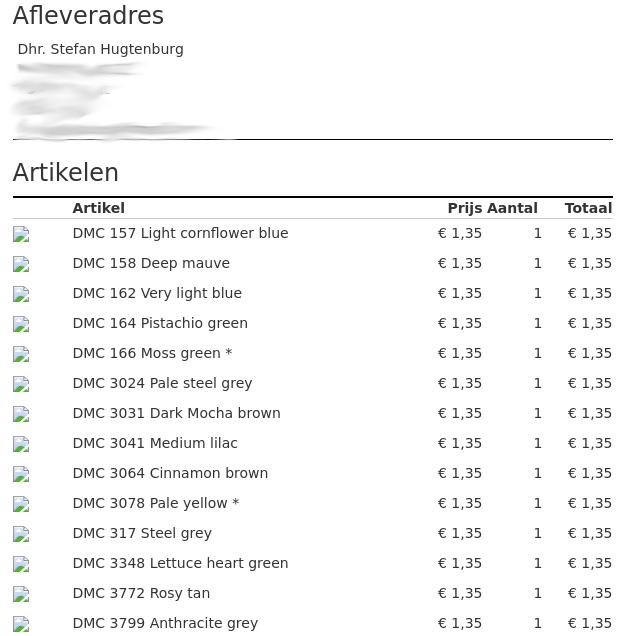
\includegraphics[width=0.8\textwidth]{figures/list.png}\\
		\hspace*{15pt}\hbox{\scriptsize Screenshot By:\thinspace{\itshape Stefan Hugtenburg}}
	\end{center}
\end{frame}

\begin{frame}
	\frametitle{Why study the list?}
	\begin{questionblock}{Use cases}
		What do we use lists for?	
	\end{questionblock}
	\pause
	\begin{answerblock}{Many things!}
		\begin{itemize}
			\item To store a collection of data.
				\pause
			\item To build other more complex/refined data structures!
		\end{itemize}
	\end{answerblock}
\end{frame}

\begin{frame}
	\frametitle{Lists in Python}
	\begin{questionblock}{Lists in Python}
		How do lists in Python work?
	\end{questionblock}
	\pause
	\begin{answerblock}{Arrays}
		They are array-based!
	\end{answerblock}
	\pause
	\begin{questionblock}{Arrays?}
		So what's an array then?
	\end{questionblock}
\end{frame}

\begin{frame}
	\frametitle{Arrays}
	\begin{block}{Array}
		An array is a block of memory of fixed size that can hold multiple items of data.
	\end{block}	
	\pause
	\begin{columns}
		\column{0.455\textwidth}
		\vspace{10pt}
		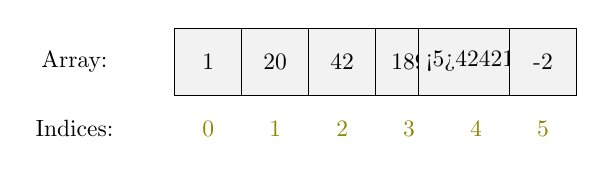
\begin{tikzpicture}[scale=0.85, transform shape]
	\foreach \x/\val in {0/1,1/20,2/42,3/189,4/\alt<5>{\alert{4242}}{17},5/-2}{
	\node[draw,rectangle, fill=gray!10, minimum size =1cm] (c) at (\x,0) {\val};
	\node[olive] (index) at (\x,-1) {\x};
}
\node[] at (-2,0) {Array:};
\node[] at (-2,-1) {Indices:};
\end{tikzpicture}

		\column{0.455\textwidth}
		\pause
		\begin{onlyenv}<3>

			\lstinputlisting{code/array.py}
		\end{onlyenv}
		\begin{onlyenv}<4>

			\lstinputlisting{code/array2.py}
		\end{onlyenv}
		\begin{onlyenv}<5->

			\lstinputlisting{code/array3.py}
		\end{onlyenv}
	\end{columns}
	\only<6>{
		\begin{questionblock}{How is this different?}
			How does this differ from a list?
		\end{questionblock}
	}
	\only<7>{
		\begin{answerblock}{Several ways}
			\begin{itemize}
				\item It's just memory, no things like \texttt{a.sort()}.
				\item It is \textit{finite}!
			\end{itemize}
		\end{answerblock}
	}
\end{frame}

\begin{frame}
	\frametitle{Array-based lists}
	\begin{block}{Array-based list}
		An array-based list (like the \texttt{list} in Python) uses an array internally.
	\end{block}
	\begin{questionblock}{Growing a list?}
		How can we then grow the list (seemingly) infinitely?
		\begin{enumerate}[A.]
			\item The list uses multiple arrays stitched together.
			\item The list also has a finite size from the start, we just never notice.
			\item The list creates a new array of size $n+1$ when the array if full.
			\item The list creates a new array of size $n*2$ when the array if full.
			\item I don't know.
		\end{enumerate}
	\end{questionblock}
\end{frame}

\begin{frame}
	\frametitle{No! Bad Frankenstein!}
	\begin{alertblock}{Stitching arrays together}
		The list uses multiple arrays stitched together.
		\begin{itemize}
			\item Although technically possible, keeping track of all of it is \st{hell} not pleasant.
			\item There are also benefits to having one continuous block of memory.
				\begin{itemize}
					\item For instance spacial caching benefits (Google it, if you are intrigued ;))
				\end{itemize}
				\pause
			\item But the idea isn't a bad one per sé. Having only single items blocks, forms the basis of the list we study
				after the break!
		\end{itemize}
	\end{alertblock}	
\end{frame}

\begin{frame}
	\frametitle{Too infinity and beyond}
	\begin{alertblock}{A hidden maximum size?}
		The list also has a finite size from the start, we just never notice.
		\begin{itemize}
			\item Nope, we can grow it so long as there is memory available.
		\end{itemize}
	\end{alertblock}	
\end{frame}

\begin{frame}
	\frametitle{So... New arrays then?}
	\begin{exampleblock}{A new one!}
		When the initial array is full, we create a new one with more capacity.\\
		We copy over all existing elements into the new array\dots\\
		And we now have new space to grow!
	\end{exampleblock}	
	\pause
	\begin{questionblock}{Question}
		But by how much should we grow?	
	\end{questionblock}
	\pause
	\begin{block}{Observations}
		\begin{itemize}
			\item Adding one item, can trigger a full copy of the array...
			\item Does that make \texttt{append} an $O(n)$ operation?
		\end{itemize}
	\end{block}	
\end{frame}

\begin{frame}
	\frametitle{It depends}
	\begin{alertblock}{Just enough room}
		The list creates a new array of size $n+1$ when the array if full.
	\end{alertblock}	
	\begin{block}{Doing it often}
		What happens when we add $n$ elements to a list of size $1$?\\
		\begin{itemize}
			\item Every time we need to copy the full list.
			\item So $O(\sum\limits_{i=1}^{n}i)$ time in total.
			\item So $O(n^2)$ to add $n$ elements\dots
		\end{itemize}
	\end{block}	
\end{frame}

\begin{frame}
	\frametitle{It depends}
	\begin{answerblock}{More than enough room}
		The list creates a new array of size $n*2$ when the array if full.
	\end{answerblock}	
	\begin{block}{Doing it often}
		What happens when we add $n$ elements?
	\end{block}
\end{frame}

\begin{frame}
	\frametitle{Amortised run time}
	\begin{block}{Amortised run time}
		Some operations have varying run times, but can be shown to be efficient when repeated multiple times. We call
		this an amortised run time.
	\end{block}	
	\pause
	\begin{exampleblock}{Consider...}
		\small
		\begin{itemize}
			\item Consider a list of size $1$ and we add $n$ elements to it.
				\vspace{-5pt}
				\pause
			\item This means we double the size of the list $\log_2(n)$ times.
				\vspace{-5pt}
				\pause
			\item This means that in total we have: $O(n)$ time to add all elements.
				\vspace{-5pt}
				\pause
			\item And $O\left(\sum\limits_{i=1}^{\log_2(n)} 2^i\right)$ operations to copy when the list grows.
				\vspace{-5pt}
			\item This geometric sequence gets us to: $O(2^{\log_2(n)}) = O(n)$ operations.
				\vspace{-5pt}
				\pause
			\item So $O(n)$ to add $n$ items!
				\vspace{-5pt}
		\end{itemize}
		\pause
		We call this an amortised run time of $O(1)$ for the append operation!
	\end{exampleblock}	
\end{frame}

\begin{frame}
	\frametitle{Inserter}
	\begin{center}
		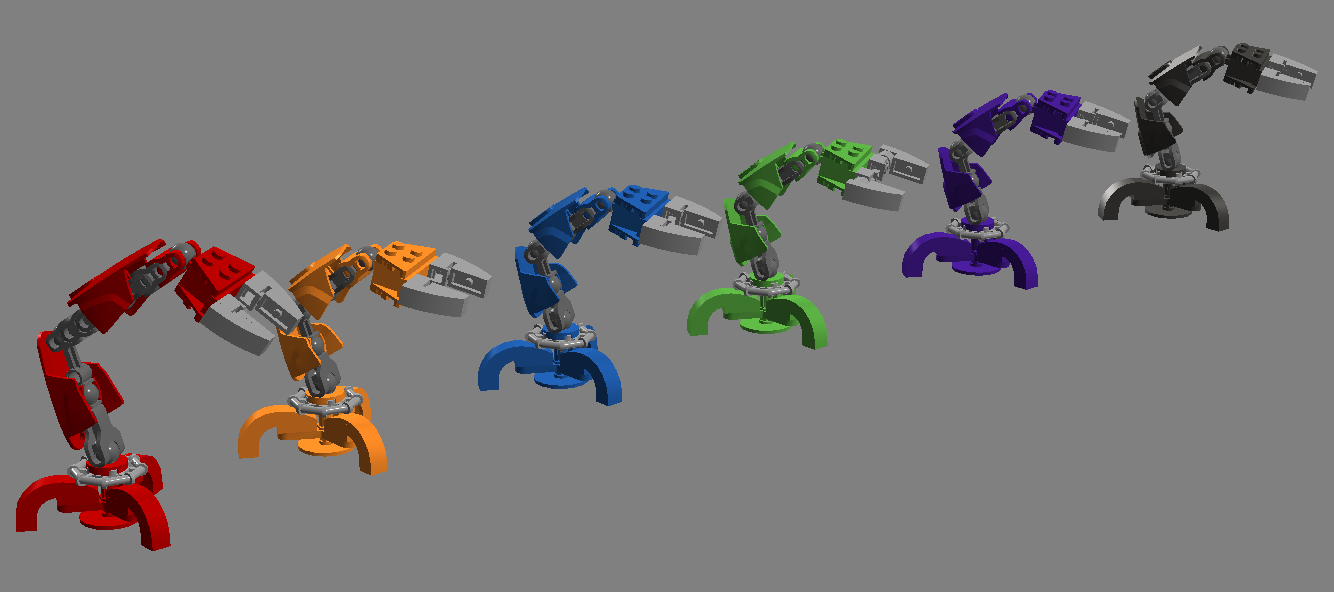
\includegraphics[width=0.8\textwidth]{figures/inserter.png}\\
		\hspace*{15pt}\hbox{\scriptsize Image By:\thinspace{\itshape TheMugbearer}}
		% https://www.reddit.com/r/factorio/comments/4s015w/decided_to_also_post_a_sort_of_factorio_fanart/
	\end{center}
\end{frame}

\begin{frame}
	\frametitle{Inserting}
	\begin{columns}
		\column{0.455\textwidth}

		\begin{questionblock}{Let's insert}
			What is the time complexity of \texttt{l.insert(index,value)} when \texttt{len(l)}=n?
			\begin{enumerate}[A.]
				\item $O(1)$
				\item $O(\textit{index})$
				\item $O(n - \textit{index})$
				\item $O(n)$
				\item $O(n^2)$
				\item I don't know.
			\end{enumerate}
		\end{questionblock}
		\pause
		\column{0.455\textwidth}
		\begin{answerblock}{Let's insert}
			We need to shift all elements after \texttt{index}, so $O(n-\textit{index})$
		\end{answerblock}
		\pause
		\begin{alertblock}{Inserting at the front}
			This means prepending is $O(n)$ for array-based lists!
		\end{alertblock}	
	\end{columns}
\end{frame}

\begin{frame}
	\frametitle{Getting rid of the trash}
	\begin{center}
		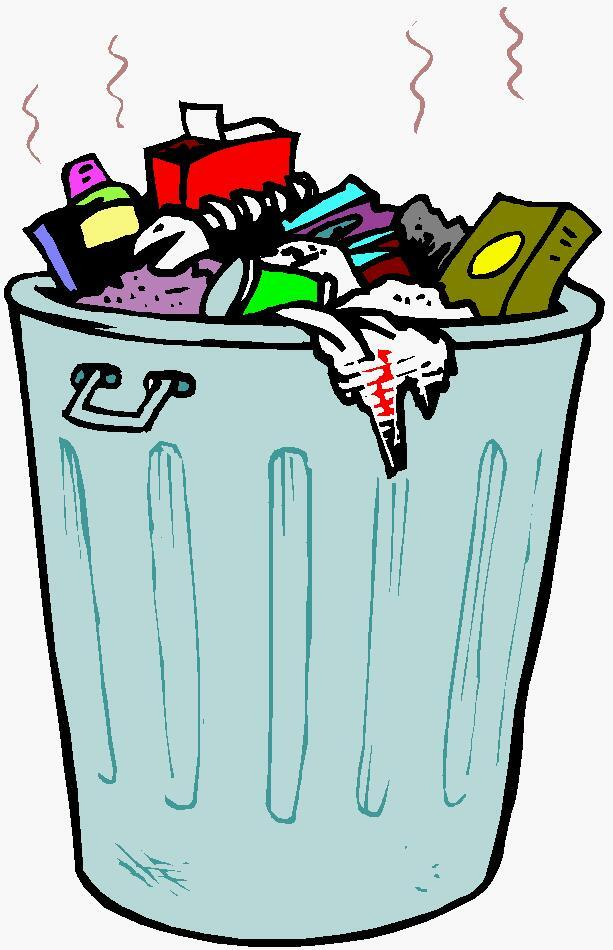
\includegraphics[width=0.3\textwidth]{figures/trash.jpg}\\
		\hspace*{15pt}\hbox{\scriptsize Image By:\thinspace{\itshape Tgasser}}
		% https://commons.wikimedia.org/wiki/File:Trash_person.jpg
	\end{center}
\end{frame}

\begin{frame}
	\frametitle{Removing an item}
	\begin{columns}
		\column{0.455\textwidth}
		\begin{questionblock}{Let's pop}
			What is the time complexity of \texttt{l.pop(index)} when \texttt{len(l)}=n?
			\begin{enumerate}[A.]
				\item $O(1)$
				\item $O(\textit{index})$
				\item $O(n - \textit{index})$
				\item $O(n)$
				\item $O(n^2)$
				\item I don't know.
			\end{enumerate}
		\end{questionblock}
		\pause
		\column{0.455\textwidth}
		\begin{answerblock}{Let's pop}
			We need to shift all elements after \texttt{index}, so $O(n-\textit{index})$.
		\end{answerblock}
		\pause
		\begin{alertblock}{Inserting at the front}
			This means removing the first item is $O(n)$ for array-based lists!
		\end{alertblock}	
	\end{columns}
\end{frame}

\begin{frame}
	\frametitle{Removing an item}
	\begin{columns}
		\column{0.455\textwidth}
		\begin{questionblock}{Let's remove}
			What is the time complexity of \texttt{l.remove(value)} when \texttt{len(l)}=n?
			\begin{enumerate}[A.]
				\item $O(1)$
				\item $O(\textit{index})$, where index is the index of the value.
				\item $O(n - \textit{index})$, where index is the index of the value.
				\item $O(n)$
				\item $O(n^2)$
				\item I don't know.
			\end{enumerate}
		\end{questionblock}
		\pause
		\column{0.455\textwidth}
		\begin{answerblock}{Let's remove}
			We need to find the element so $O(\textit{index})$.\\
			We need to shift all elements after \texttt{index}, so $O(n-\textit{index})$.\\
			Together this is $O(n)$.
		\end{answerblock}
	\end{columns}
\end{frame}

\begin{frame}
	\frametitle{Freeing up memory}
	\begin{block}{Freeing up space}
		When we remove sufficient items, we can free up space again.\\
		We do this when 25\% of the capacity is used.
	\end{block}	
	\pause
	\begin{questionblock}{Why 25\%?}
		Why not just when we drop below 50\% again?
	\end{questionblock}
	\pause
	\begin{answerblock}{Thrashing}
		Thrashing is repeatedly claiming and releasing memory (and in this case copying the array).\\
		To avoid this, we use a different bound on when we release memory.
	\end{answerblock}
\end{frame}

\begin{frame}
	\frametitle{Lists in Python}
	So to summarise:
	\begin{itemize}
		\item Insert first element: $O(n)$.
		\item Insert at index $k$: $O(n-k)$.
		\item Append: amortised $O(1)$.
		\item Remove first element: $O(n)$.
		\item Remove last element: amortised $O(1)$.
		\item Remove index $k$: $O(n-k)$.
		\item Search (discussed last week): $O(n)$.
	\end{itemize}
\end{frame}
